\documentclass[a4paper,12pt]{article}
\usepackage[top = 2.5cm, bottom = 2.5cm, left = 2.5cm, right = 2.5cm]{geometry} 
\usepackage[T1]{fontenc}
\usepackage[utf8]{inputenc}
\usepackage{multirow}
\usepackage{booktabs}
\usepackage{graphicx} 
\usepackage{setspace}
\setlength{\parindent}{0in}
\usepackage{float}
\usepackage{fancyhdr}
\usepackage[table,xcdraw]{xcolor}
\pagestyle{fancy}
\fancyhf{}
\lhead{\footnotesize GEO1001: Homework 1}
\rhead{\footnotesize Georgios Triantafyllou (5381738)}
\cfoot{\footnotesize \thepage} 

\begin{document}
	\thispagestyle{empty}
	\begin{tabular}{p{15.5cm}}
		{\large \bf Sensing Technologies and Mathematics for Geomatics} \\
		GEO1001.2020 \\ MSc Geomatics \\ Delft University of Technology \\
		\hline
	\end{tabular} 
\vspace*{0.3cm}
\begin{center}
	{\Large \bf Homework 1}
	\vspace{2mm}
	{\bf Georgios Triantafyllou (5381738)}
\end{center} 
\vspace{0.4cm}
\section{A1}
 \subsection{A1.1}
From the results i have there no many things that i could say.
 \subsection{A1.2}
The number of bins it is really important because if we use too few number of bins, the histogram does not really portray the data very well (Figure 1). From the other side if we have too many bins, we get a broken comb look, which also does not give a good sense of the distribution (Figure 2). A good example is visible in to the next histograms.
%\begin{verbatim}
%	If you have code put it here
%\end{verbatim}
  \begin{figure}[H] 
	\centering
	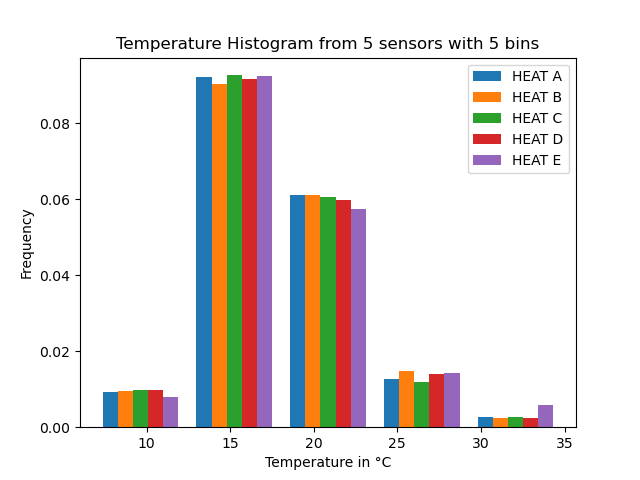
\includegraphics[width=0.7\textwidth]{Temperature Histogram from 5 sensors with 5 bins.png}
	\caption{Temperature Histogram from 5 sensors with 5 bins}\cite{Maiullari2020}
  \end{figure}
  \begin{figure}[H] 
	\centering
	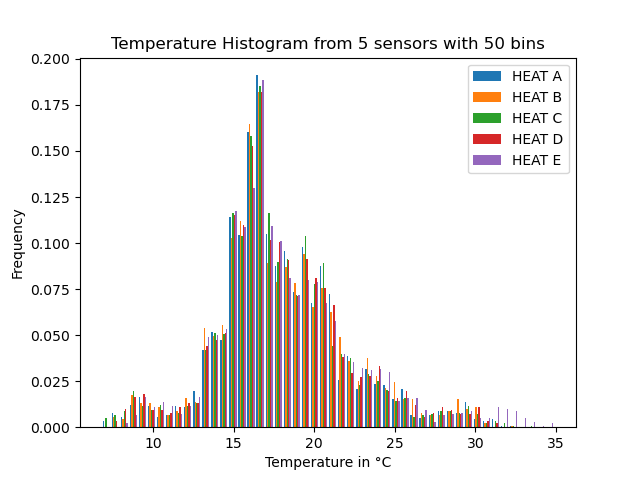
\includegraphics[width=0.7\textwidth]{Temperature Histogram from 5 sensors with 50 bins.png}
	\caption{Temperature Histogram from 5 sensors with 50 bins}\cite{Maiullari2020}
  \end{figure}

 \subsection{A1.3}
  \begin{figure}[H] 
	\centering
	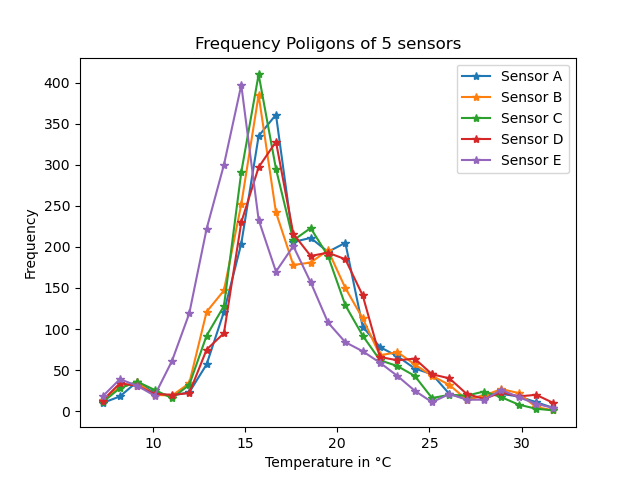
\includegraphics[width=0.7\textwidth]{Frequency Poligons of 5 Sensors.png}
	\caption{Frequency Poligons of 5 Sensors}\cite{Maiullari2020}
  \end{figure}

 \subsection{A1.4}
  \begin{figure}[H] 
	\centering
	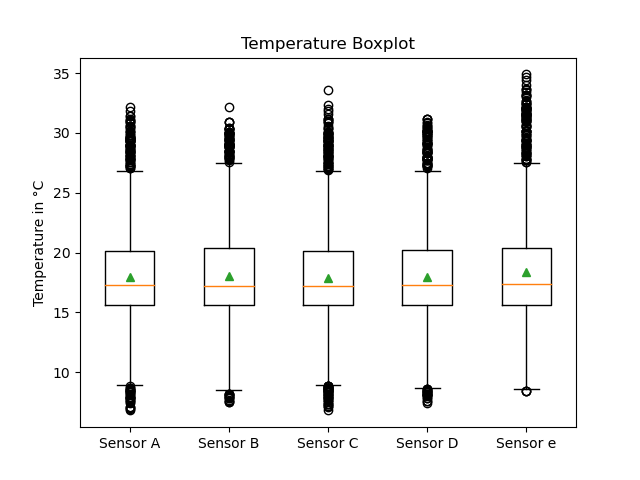
\includegraphics[width=0.7\textwidth]{Temperature Boxplot.png}
	\caption{Temperature Boxplot}\cite{Maiullari2020}
  \end{figure}
  \begin{figure}[H] 
	\centering
	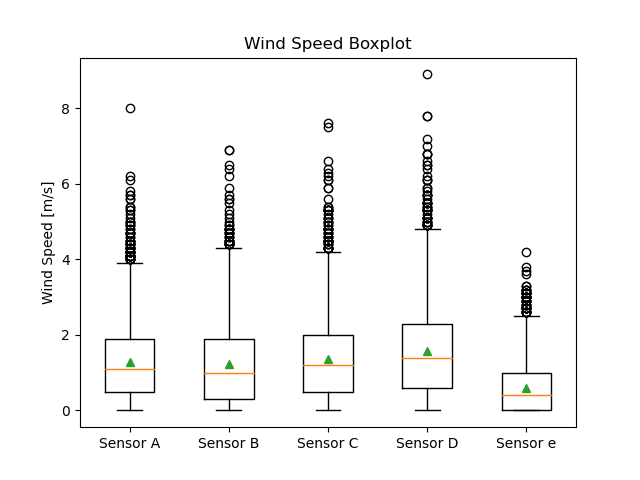
\includegraphics[width=0.7\textwidth]{Wind Speed Boxplot.png}
	\caption{Wind Speed Boxplot}\cite{Maiullari2020}
  \end{figure}
  \begin{figure}[H] 
	\centering
	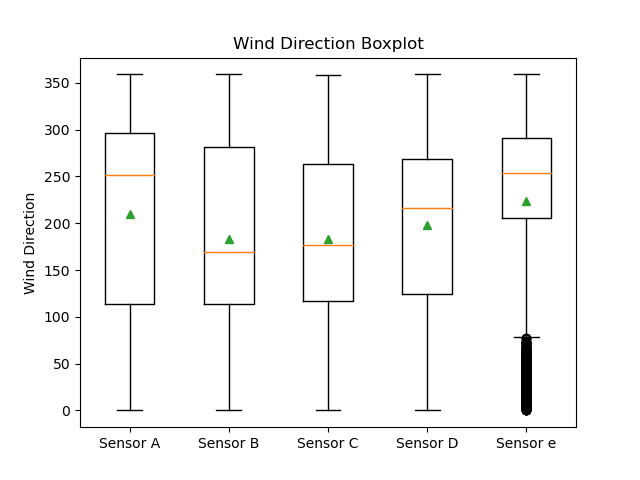
\includegraphics[width=0.7\textwidth]{Wind Direction Boxplot.png}
	\caption{Wind Direction Boxplot}\cite{Maiullari2020}
  \end{figure}

\section{A2}
 \subsection{A2.1}
 From the the figures below we can realize that the behavior of the distributions for each Sensor's Temperature look pretty similar. 
  \begin{figure}[H] 
	\centering
	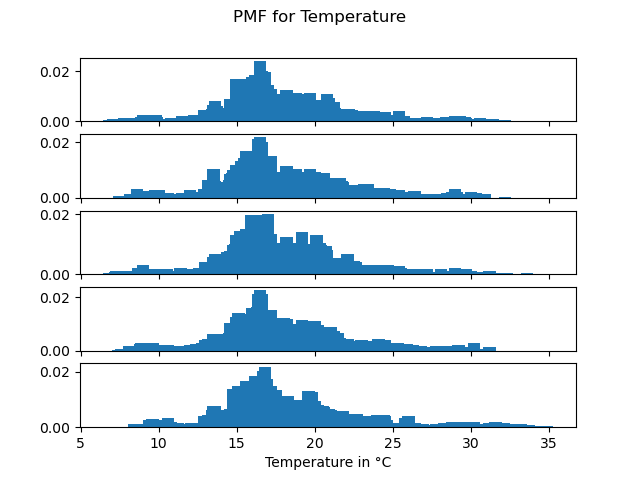
\includegraphics[width=0.7\textwidth]{PMF for Temperature.png}
	\caption{PMF for Temperature}\cite{Maiullari2020}
  \end{figure}
  \begin{figure}[H] 
	\centering
	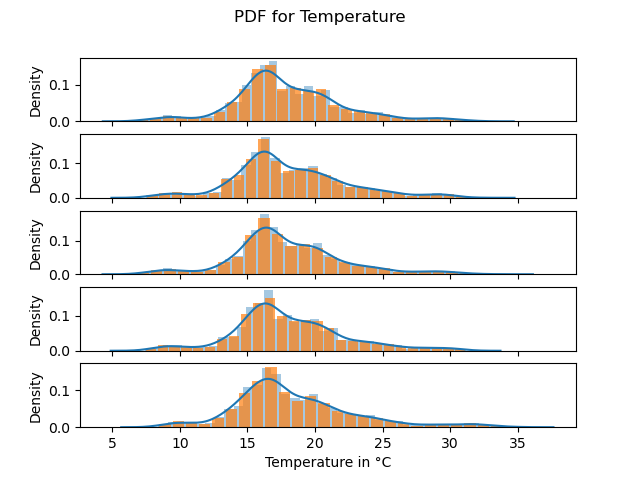
\includegraphics[width=0.7\textwidth]{PDF for Temperature.png}
	\caption{PDF for Temperature}\cite{Maiullari2020}
  \end{figure}
  \begin{figure}[H] 
	\centering
	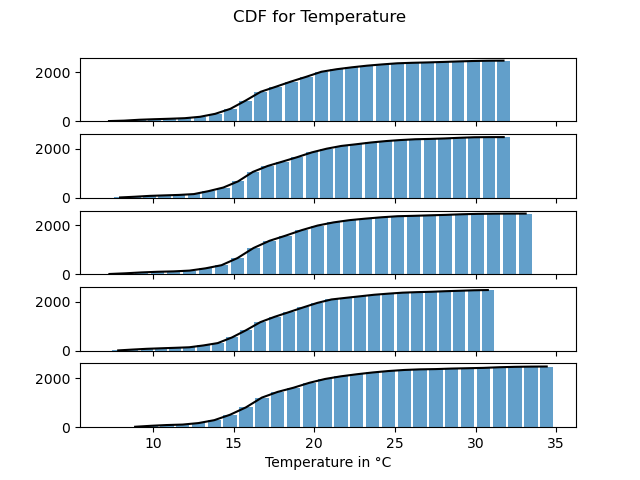
\includegraphics[width=0.7\textwidth]{CDF for Temperature.png}
	\caption{CDF for Temperature}\cite{Maiullari2020}
  \end{figure}
 \subsection{A2.2}
 From the figures below we can see that there is no actual diference between the PDF and the Kernel Density Estimation (KDE) for the Wind Speed and that happens because the KDE is actually an algorithm that takes a sample
 and finds an appropriately smooth PDF that fits the data. So the only diference is that the KDE shows less information in the graph and makes it easier for the audience to understand it.
  \begin{figure}[H] 
	\centering
	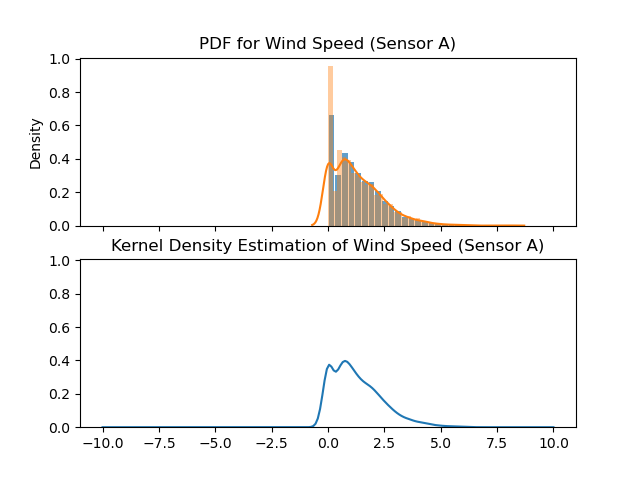
\includegraphics[width=0.7\textwidth]{PDF for Wind Speed (Sensor A).png}
	\caption{PDF for Wind Speed (Sensor A)}\cite{Maiullari2020}
  \end{figure}
  \begin{figure}[H] 
	\centering
	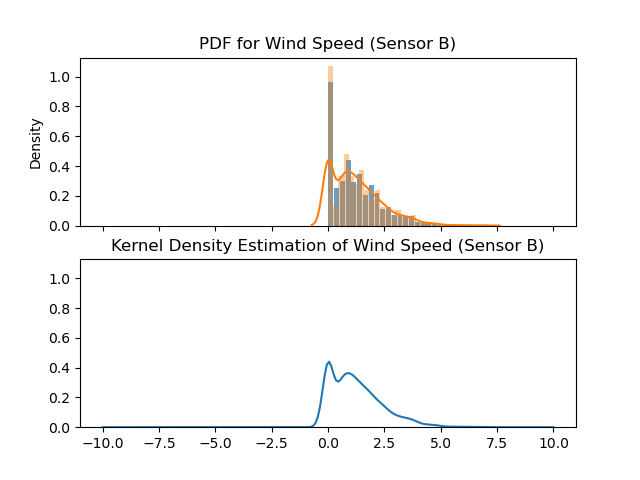
\includegraphics[width=0.7\textwidth]{PDF for Wind Speed (Sensor B).png}
	\caption{PDF for Wind Speed (Sensor B)}\cite{Maiullari2020}
  \end{figure}
  \begin{figure}[H] 
	\centering
	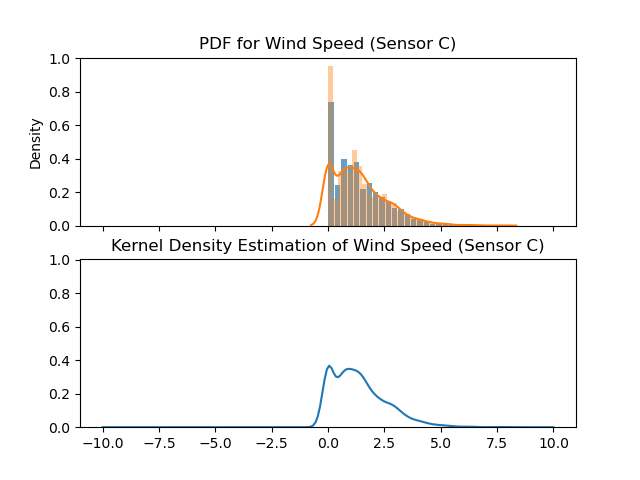
\includegraphics[width=0.7\textwidth]{PDF for Wind Speed (Sensor C).png}
	\caption{PDF for Wind Speed (Sensor C)}\cite{Maiullari2020}
  \end{figure}
  \begin{figure}[H] 
	\centering
	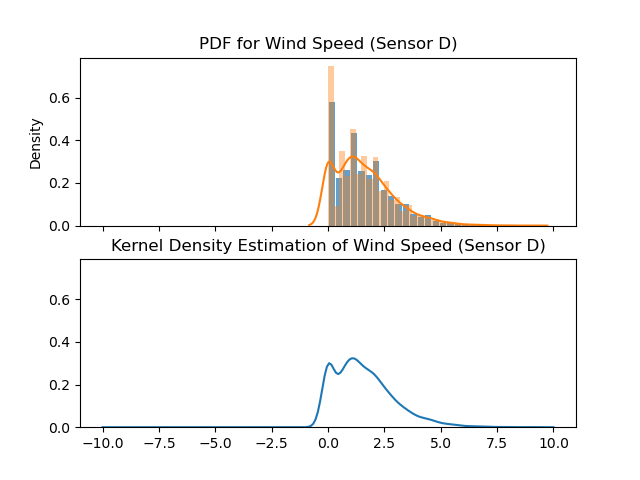
\includegraphics[width=0.7\textwidth]{PDF for Wind Speed (Sensor D).png}
	\caption{PDF for Wind Speed (Sensor D)}\cite{Maiullari2020}
  \end{figure}
  \begin{figure}[H] 
	\centering
	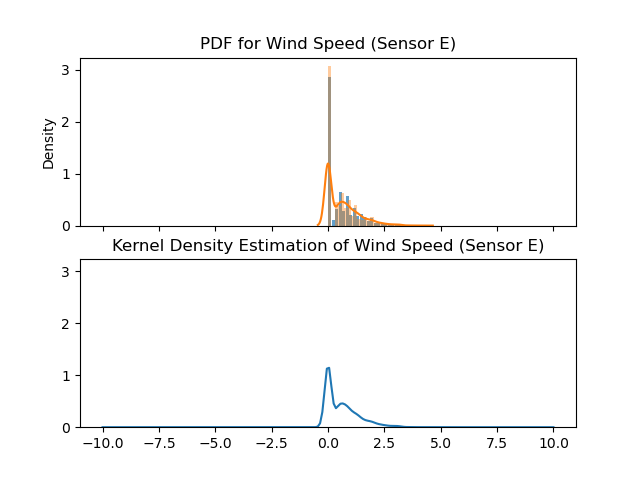
\includegraphics[width=0.7\textwidth]{PDF for Wind Speed (Sensor E).png}
	\caption{PDF for Wind Speed (Sensor E)}\cite{Maiullari2020}
  \end{figure}
\section{A3}
 \subsection{A3.1}
\begin{table}[]
 	\centering
 	\begin{tabular}{llll}
 		\hline
 		\multicolumn{1}{|l|}{Sensors Relationships} & \multicolumn{1}{l|}{Variables}   & \multicolumn{1}{l|}{Pearson Coefficient} & \multicolumn{1}{l|}{Spearman Coefficient} \\ \hline
 		\multicolumn{1}{|c|}{}                      & \multicolumn{1}{l|}{Temperature} & \multicolumn{1}{l|}{0.98810313}          & \multicolumn{1}{l|}{0.987378955}          \\ \hline
 		\multicolumn{1}{|c|}{AB}                    & \multicolumn{1}{l|}{Crosswind}   & \multicolumn{1}{l|}{0.550352585}         & \multicolumn{1}{l|}{0.596982562}          \\ \hline
 		\multicolumn{1}{|l|}{}                      & \multicolumn{1}{l|}{WBGT}        & \multicolumn{1}{l|}{0.991259553}         & \multicolumn{1}{l|}{0.992132436}          \\ \hline
 		& Temperature                      & 0.988608719                              & 0.988292007                               \\
 		\multicolumn{1}{c}{AC}                      & Crosswind                        & 0.51405088                               & 0.577228891                               \\
 		& WBGT                             & 0.99189585                               & 0.992472018                               \\ \hline
 		\multicolumn{1}{|l|}{}                      & \multicolumn{1}{l|}{Temperature} & \multicolumn{1}{l|}{0.985613462}         & \multicolumn{1}{l|}{0.984627239}          \\ \hline
 		\multicolumn{1}{|c|}{AD}                    & \multicolumn{1}{l|}{Crosswind}   & \multicolumn{1}{l|}{0.489895013}         & \multicolumn{1}{l|}{0.601889059}          \\ \hline
 		\multicolumn{1}{|l|}{}                      & \multicolumn{1}{l|}{WBGT}        & \multicolumn{1}{l|}{0.987013949}         & \multicolumn{1}{l|}{0.988291923}          \\ \hline
 		& Temperature                      & 0.969204792                              & 0.9717698                                 \\
 		\multicolumn{1}{c}{AD}                      & Crosswind                        & 0.465124685                              & 0.537844665                               \\
 		& WBGT                             & 0.949828692                              & 0.949127535                               \\ \hline
 		\multicolumn{1}{|l|}{}                      & \multicolumn{1}{l|}{Temperature} & \multicolumn{1}{l|}{0.98448517}          & \multicolumn{1}{l|}{0.985440109}          \\ \hline
 		\multicolumn{1}{|c|}{BC}                    & \multicolumn{1}{l|}{Crosswind}   & \multicolumn{1}{l|}{0.516102417}         & \multicolumn{1}{l|}{0.590683619}          \\ \hline
 		\multicolumn{1}{|l|}{}                      & \multicolumn{1}{l|}{WBGT}        & \multicolumn{1}{l|}{0.989729694}         & \multicolumn{1}{l|}{0.989863576}          \\ \hline
 		& Temperature                      & 0.986265403                              & 0.986048723                               \\
 		\multicolumn{1}{c}{BD}                      & Crosswind                        & 0.488029338                              & 0.604818597                               \\
 		& WBGT                             & 0.987864209                              & 0.987374811                               \\ \hline
 		\multicolumn{1}{|l|}{}                      & \multicolumn{1}{l|}{Temperature} & \multicolumn{1}{l|}{0.972089738}         & \multicolumn{1}{l|}{0.976859613}          \\ \hline
 		\multicolumn{1}{|c|}{BE}                    & \multicolumn{1}{l|}{Crosswind}   & \multicolumn{1}{l|}{0.39214871}          & \multicolumn{1}{l|}{0.500281016}          \\ \hline
 		\multicolumn{1}{|l|}{}                      & \multicolumn{1}{l|}{WBGT}        & \multicolumn{1}{l|}{0.95440893}          & \multicolumn{1}{l|}{0.956900474}          \\ \hline
 		& Temperature                      & 0.988742872                              & 0.988185589                               \\
 		\multicolumn{1}{c}{CD}                      & Crosswind                        & 0.562888199                              & 0.635906168                               \\
 		& WBGT                             & 0.991820559                              & 0.991421934                               \\ \hline
 		\multicolumn{1}{|l|}{}                      & \multicolumn{1}{l|}{Temperature} & \multicolumn{1}{l|}{0.972097215}         & \multicolumn{1}{l|}{0.977342412}          \\ \hline
 		\multicolumn{1}{|c|}{CE}                    & \multicolumn{1}{l|}{Crosswind}   & \multicolumn{1}{l|}{0.473233228}         & \multicolumn{1}{l|}{0.532232093}          \\ \hline
 		\multicolumn{1}{|l|}{}                      & \multicolumn{1}{l|}{WBGT}        & \multicolumn{1}{l|}{0.949269532}         & \multicolumn{1}{l|}{0.949345587}          \\ \hline
 		& Temperature                      & 0.971365706                              & 0.975848255                               \\
 		\multicolumn{1}{c}{DE}                      & Crosswind                        & 0.465192078                              & 0.527325327                               \\
 		& WBGT                             & 0.948090212                              & 0.94870202                               
 	\end{tabular}
 	\caption{Correlations between all the sensors for the variables: Temperature, Wet Bulb Globe Temperature (WBGT), Crosswind Speed}\cite{Maiullari2020}
\end{table}
   \begin{figure}[H] 
 	\centering
 	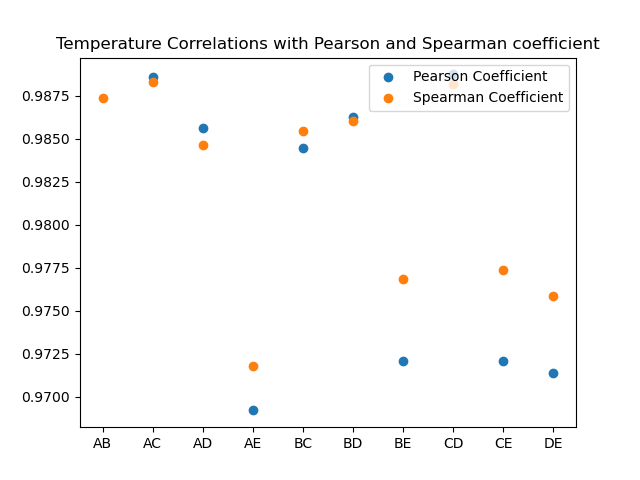
\includegraphics[width=0.7\textwidth]{Temperature Correlations with P and Sp coeff.png}
 	\caption{Temperature Correlations with P and Sp coeff}\cite{Maiullari2020}
 \end{figure}
 \begin{figure}[H] 
 	\centering
 	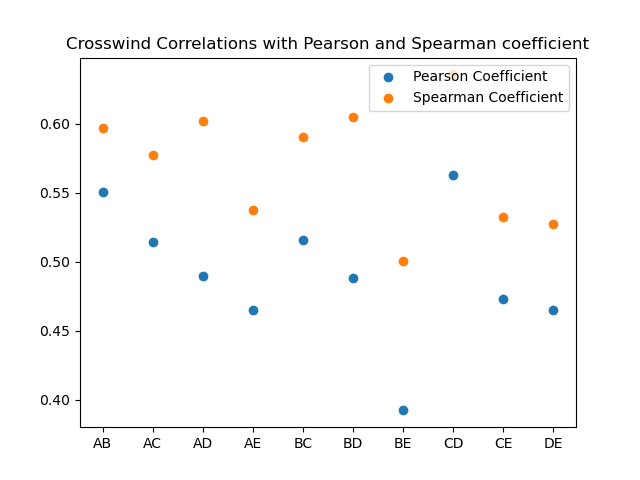
\includegraphics[width=0.7\textwidth]{Crosswind Correlations with P and Sp coeff.png}
 	\caption{Crosswind Correlations with P and Sp coeff}\cite{Maiullari2020}
 \end{figure}
 \begin{figure}[H] 
 	\centering
 	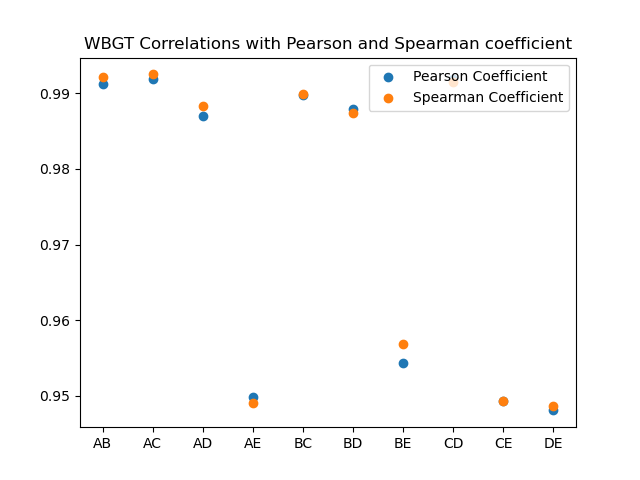
\includegraphics[width=0.7\textwidth]{WBGT Correlations with P and Sp coeff.png}
 	\caption{WBGT Correlations with P and Sp coeff}\cite{Maiullari2020}
 \end{figure}
 \subsection{A3.2}
That mostly they have high correlation since most of them are really near to 1 as about the Temperature and WBGT and not so high about Crosswind since the correlation is aroun 0.5.
 \subsection{A3.3}
 With a look in the correlations of the sensors we could say that 
\begin{figure}[H] 
	\centering
	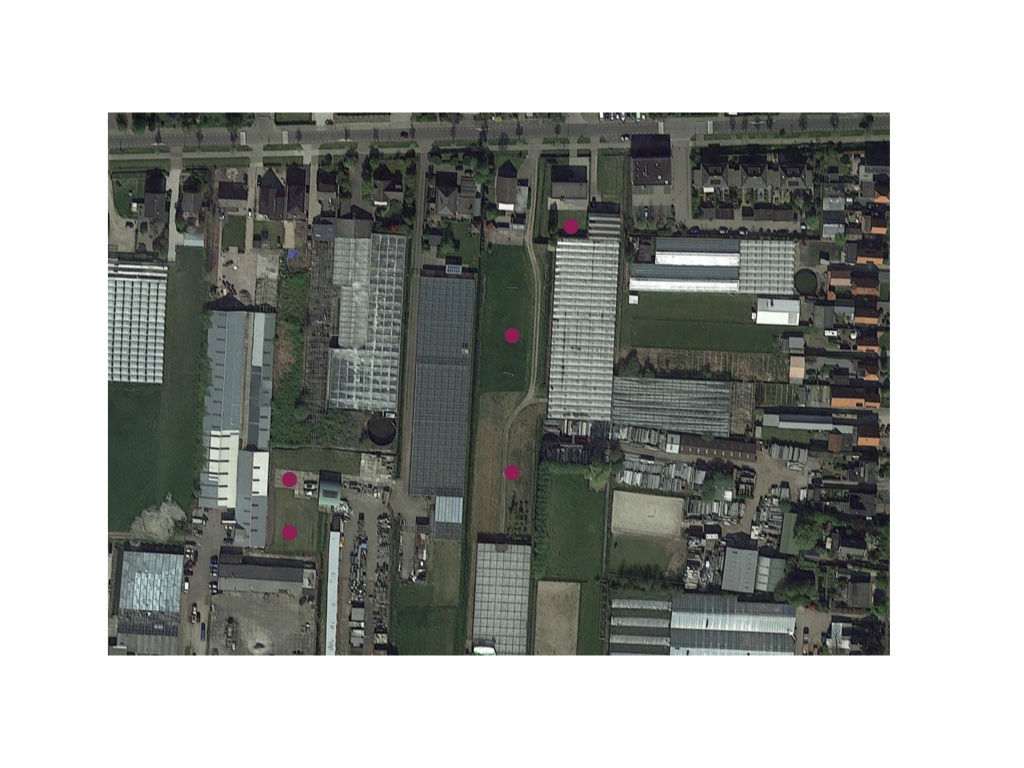
\includegraphics[width=0.9\textwidth]{Sensors Location.png}
	\caption{Sensors Location}
\end{figure}
\section{A4}
 \subsection{A4.1}
   \begin{figure}[H] 
 	\centering
 	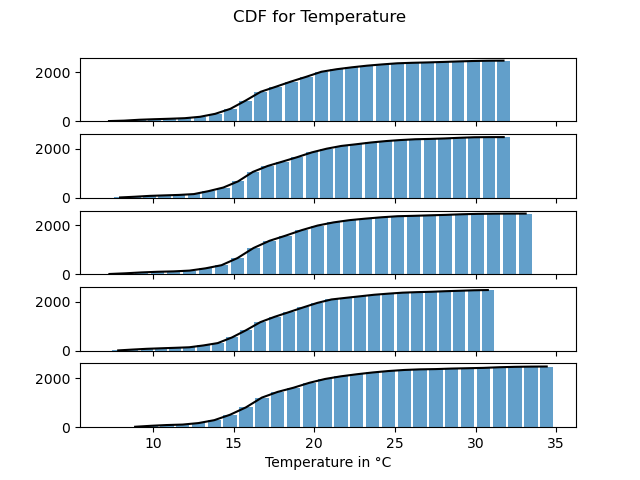
\includegraphics[width=0.7\textwidth]{CDF for Temperature.png}
 	\caption{CDF for Temperature}\cite{Maiullari2020}
   \end{figure}
   \begin{figure}[H] 
	\centering
	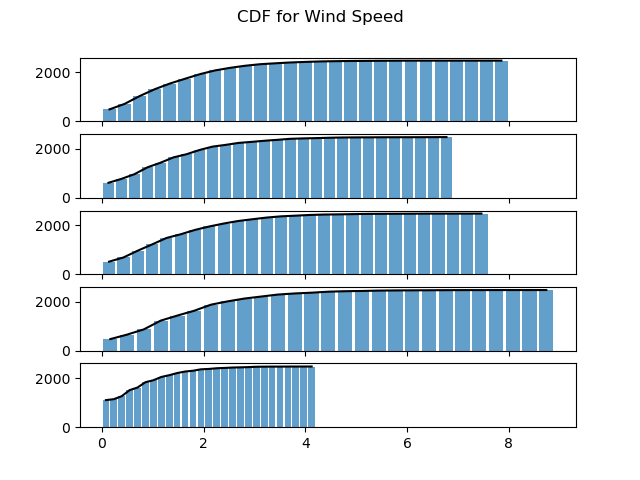
\includegraphics[width=0.7\textwidth]{CDF for Wind Speed.png}
    \caption{CDF for Wind Speed}\cite{Maiullari2020}
   \end{figure}
\subsection{A4.2-3}
So in the Table 3 above is visible the p-values from the requested sensors. We can conclude that most of them as about the temperature values (3 out of 4) are way above the 0.05 so we reject the Hypothesis. And totally the opposite is happening with the Wind speed.
\begin{table}[]
	\centering
	\begin{tabular}{|l|r|r|r|c|}
		\hline
		\multirow{2}{*}{Variables}                         & \multicolumn{3}{c|}{Confidence Intervals}                                    & \multicolumn{1}{l|}{\multirow{2}{*}{Sensors}} \\ \cline{2-4}
		& \multicolumn{1}{l|}{m-h} & \multicolumn{1}{l|}{m} & \multicolumn{1}{l|}{m+h} & \multicolumn{1}{l|}{}                         \\ \hline
		\multicolumn{1}{|c|}{\multirow{5}{*}{Temperature}} & 17.8121                  & 17.9691                & 18.1261                  & A                                             \\ \cline{2-5} 
		\multicolumn{1}{|c|}{}                             & 17.9047                  & 18.0654                & 18.2261                  & B                                             \\ \cline{2-5} 
		\multicolumn{1}{|c|}{}                             & 17.7549                  & 17.9131                & 18.0713                  & C                                             \\ \cline{2-5} 
		\multicolumn{1}{|c|}{}                             & 17.8381                  & 17.9964                & 18.1546                  & D                                             \\ \cline{2-5} 
		\multicolumn{1}{|c|}{}                             & 18.1819                  & 18.3539                & 18.5259                  & E                                             \\ \hline
		\multirow{5}{*}{Wind Speed}                        & 1.2462                   & 1.2903                 & 1.3344                   & A                                             \\ \cline{2-5} 
		& 1.1972                   & 1.2421                 & 1.2871                   & B                                             \\ \cline{2-5} 
		& 1.3243                   & 1.3715                 & 1.4186                   & C                                             \\ \cline{2-5} 
		& 1.5297                   & 1.5817                 & 1.6337                   & D                                             \\ \cline{2-5} 
		& 0.5681                   & 0.5962                 & 0.6244                   & E                                             \\ \hline
	\end{tabular}
	\caption{95/100 confidence intervals for variables Temperature and Wind Speed for all the sensors}\cite{Maiullari2020}
\end{table}
\begin{table}[]
	\centering
	\begin{tabular}{|c|r|r|c|}
		\hline
		\multicolumn{1}{|l|}{Sensors} & \multicolumn{1}{l|}{Student Test} & \multicolumn{1}{l|}{p value} & \multicolumn{1}{l|}{Variables} \\ \hline
		ED                            & 3.00023                           & 0.00271                      & \multirow{4}{*}{Temperature}   \\ \cline{1-3}
		DC                            & 0.72939                           & 0.46580                      &                                \\ \cline{1-3}
		CB                            & -1.32423                          & 0.18549                      &                                \\ \cline{1-3}
		BA                            & 0.84084                           & 0.40048                      &                                \\ \hline
		ED                            & -32.67317                         & 0.00000                      & \multirow{4}{*}{Wind Speed}    \\ \cline{1-3}
		DC                            & 5.87115                           & 0.00000                      &                                \\ \cline{1-3}
		CB                            & 3.89266                           & 0.00010                      &                                \\ \cline{1-3}
		BA                            & -1.50061                          & 0.13352                      &                                \\ \hline
	\end{tabular}
	\caption{Student Test and p-values}
\end{table}
\section{Bonus Question}

\bibliographystyle{plain}

\bibliography{bibliography}
\end{document}